\documentclass[border=6pt]{standalone}
\usepackage{tikz}
\usetikzlibrary{arrows.meta,positioning,calc,shapes.geometric,fit,backgrounds,patterns,matrix,decorations.pathreplacing}
\begin{document}
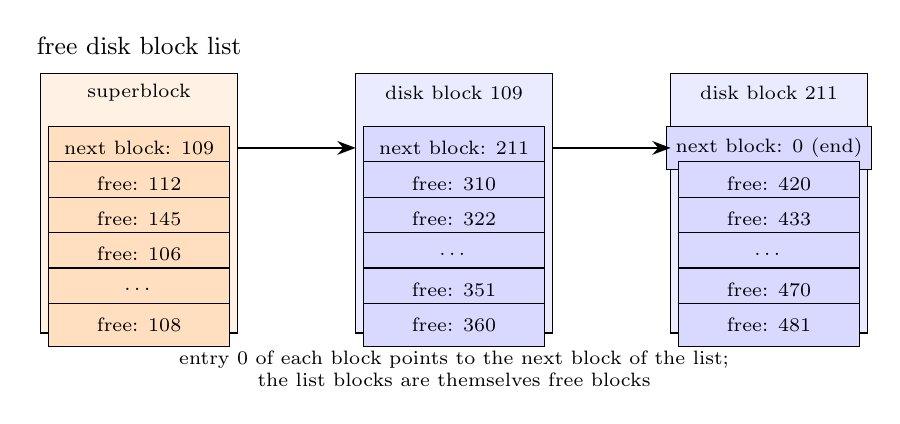
\begin{tikzpicture}[>=Stealth,font=\small]
\tikzstyle{b}=[draw,minimum height=0.55cm,minimum width=2.3cm,font=\scriptsize]
\node[font=\small] at (0,1.5) {free disk block list};
\node[draw,minimum width=2.5cm,minimum height=3.3cm,fill=orange!10] (sb) at (0,-0.5) {};
\node[font=\scriptsize] at (0,0.9) {superblock};
\foreach \i/\t in {0/{next block: 109},1/{free: 112},2/{free: 145},3/{free: 106},4/{\ldots},5/{free: 108}} \node[b,fill=orange!25] at (0,0.3-\i*0.45-0.1) {\t};
\node[draw,minimum width=2.5cm,minimum height=3.3cm,fill=blue!8] (b1) at (4,-0.5) {};
\node[font=\scriptsize] at (4,0.9) {disk block 109};
\foreach \i/\t in {0/{next block: 211},1/{free: 310},2/{free: 322},3/{\ldots},4/{free: 351},5/{free: 360}} \node[b,fill=blue!15] at (4,0.3-\i*0.45-0.1) {\t};
\node[draw,minimum width=2.5cm,minimum height=3.3cm,fill=blue!8] (b2) at (8,-0.5) {};
\node[font=\scriptsize] at (8,0.9) {disk block 211};
\foreach \i/\t in {0/{next block: 0 (end)},1/{free: 420},2/{free: 433},3/{\ldots},4/{free: 470},5/{free: 481}} \node[b,fill=blue!15] at (8,0.3-\i*0.45-0.1) {\t};
\draw[->,thick] (1.25,0.2) -- (2.75,0.2); \draw[->,thick] (5.25,0.2) -- (6.75,0.2);
\node[font=\scriptsize,align=center] at (4,-2.6) {entry 0 of each block points to the next block of the list;\\ the list blocks are themselves free blocks};
\end{tikzpicture}
\end{document}
